% LaTeX template for ECE 496 Reports
% Last updated 27 January 2014 by Ben Ujcich

%% CHANGE REPORT TITLE HERE
\newcommand{\reporttitle}{
2-Wheeled Segway Robot Design:
Preliminary Report
}

%% HEADER/PREAMBLE INFORMATION

\documentclass[11pt]{report}
\usepackage[T1]{fontenc}
\usepackage[utf8]{inputenc}

% "The font should be 11pt Times New Roman"
\usepackage{mathptmx}               

% "The body of the paper should use 1" margins on all sides."
\usepackage[margin=1in]{geometry}

% "Pages must be numbered, starting with 1 on the first page in the body of the report.
% The cover page should not be numbered. 
% Page numbers should be in the bottom-right corner of the page."
\usepackage{fancyhdr}
\pagestyle{fancy}
\fancyhead{}
\fancyfoot{}
\renewcommand{\headrulewidth}{0pt}
\fancyfoot[R]{\thepage}

% Set up customized spacing
\usepackage{setspace}

% Allows for Trademark Symbols
\usepackage{textcomp}

% Remove spacing between items in lists
\usepackage{enumitem}

% Remove extra spacing between titles of sections and subsections
\usepackage{titlesec}
\titlespacing\section{0pt}{0pt plus 4pt minus 2pt}{0pt plus 2pt minus 2pt}
\titlespacing\subsection{0pt}{0pt plus 4pt minus 2pt}{0pt plus 2pt minus 2pt}
\titlespacing\subsubsection{0pt}{0pt plus 4pt minus 2pt}{0pt plus 2pt minus 2pt}

% Set up BibTeX integration using IEEE citation format
\usepackage{cite}
\bibliographystyle{ieeetr}
\usepackage{url}

% Set bibliography to have a section header rather than chapter header
\makeatletter
\renewenvironment{thebibliography}[1]
     {\section*{Works Cited}% <-- this line was changed from \chapter* to \section*
      \@mkboth{\MakeUppercase\bibname}{\MakeUppercase\bibname}%
      \list{\@biblabel{\@arabic\c@enumiv}}%
           {\settowidth\labelwidth{\@biblabel{#1}}%
            \leftmargin\labelwidth
            \advance\leftmargin\labelsep
            \@openbib@code
            \usecounter{enumiv}%
            \let\p@enumiv\@empty
            \renewcommand\theenumiv{\@arabic\c@enumiv}}%
      \sloppy
      \clubpenalty4000
      \@clubpenalty \clubpenalty
      \widowpenalty4000%
      \sfcode`\.\@m}
     {\def\@noitemerr
       {\@latex@warning{Empty `thebibliography' environment}}%
      \endlist}
\makeatother

% Set up math
\usepackage{amsmath}
\usepackage{amsfonts}
\usepackage{amssymb}

% Set up graphics
\usepackage{graphicx}
\usepackage{float}

% Set up tables
\usepackage{tabularx}


%% START OF DOCUMENT

\begin{document}

% "The main body of text should use 1.5 spacing"
\begin{spacing}{1.5}

% Suppress page numbering on first page
\thispagestyle{empty}

% Title
% "The title should be centered and written in approximately 22pt font."
\vspace*{72pt}
{
\huge
\begin{center}
    \reporttitle
\end{center}
}
\vspace{72pt}

% Team Number
% "The Team number should be centered and written several lines below the title and should use a
% similar size font as the title."
{
\huge
\begin{center}
  Team SR03
\end{center}
}

% Team Members
% "Directly below the team identifier, team members should be listed alphabetically by last name, one
% per line, in approximately 14pt font. The column of names should be approximately centered on
% the page, but the names within the column should be left justified (so they all start at the same
% horizontal position)."
{
\Large 
\begin{center}
  \begin{tabular}{l}
    Laura Clancy \\
    Julian Coy \\
    Katelyn Fry \\
    Gregory Stephens \\
    Ben Ujcich
  \end{tabular}
\end{center}
}

% New page and reset page numbering
\clearpage
\setcounter{page}{1}

%% START EDITS BELOW %%




\section*{Problem Statement} %(0.5 pages)

The desired goal of this senior design project is to build a functioning robot that can successfully balance and move on two wheels as directed by the user. This design is meant to be based on the commercial Segway robot but created on a much smaller scale. The robot will be roughly 18 inches high and no more than 9 inches wide. Without the use of RC Servo motors, the miniature Segway robot must be able to move forwards, backwards, and turn left and right. The remote control will consist of a wireless PlayStation controller which enables all the ranges of desired motion. An individual power amplifier must be constructed and the entire device must be run from a single DC voltage supplied to the system. The system will be controlled wirelessly with Bluetooth\textsuperscript{\textregistered} communication connecting the Tiva C Series TM4C123G LaunchPad and the computer. The robot will be able to withstand perturbations and balance itself quickly and accordingly. The main test and goal for the robot will be its ability to traverse a relatively flat surface with few balancing problems. Both cordless operation and stability will be taken as the most important aspects to perfect. Stability will be stressed over speed due to the limited testing environment. 


\section*{Design Objectives} %(0.5-1 page)

\subsection*{Performance Goals}

Certain goals take precedence in this project: cordless operation and stability. Cordless operation will not only create a seamless and efficient look but will also greatly reduce risks concerning tangling wires around the robot during motion. The implementation of the Bluetooth\textsuperscript{\textregistered} and battery systems will enable this. Additionally, we desire that the robot should be extremely stable and be able to balance itself with minimal movements and overshoots. Ideally, it would be stable enough to place something on top without falling during movement and testing. To make this achievable, the motors must be capable of exerting high torque on the wheels at quick response times. For this goal, the gyroscope will use three axes of motion to maximize the efficiency of the controls that direct the motors. Lastly, utilizing the voltage regulator and power amplifier will ensure that all the electronics and controller receive the proper power to function as desired.

\subsection*{Design Principles}

\begin{itemize}[noitemsep,nolistsep]
    \item \emph{Choose off-the-shelf parts} rather than self-made parts whenever possible.
    \item \emph{Reuse and expand on open-source software libraries} to avoid spending time writing code that duplicates functionality that already exists elsewhere (and is likely more robust).
    \item \emph{Keep the hardware simple} by using the least amount of hardware necessary for operation to avoid additional potential points of failure.
    \item \emph{Modularize systems and components}. Each component should do one thing and do it well.
\end{itemize}


\section*{Preliminary Design} %(3-5 pages)

Figure \ref{BlockDiagram} shows a block diagram of the subsystems used in our design.

\begin{figure}[H]
    \centering
    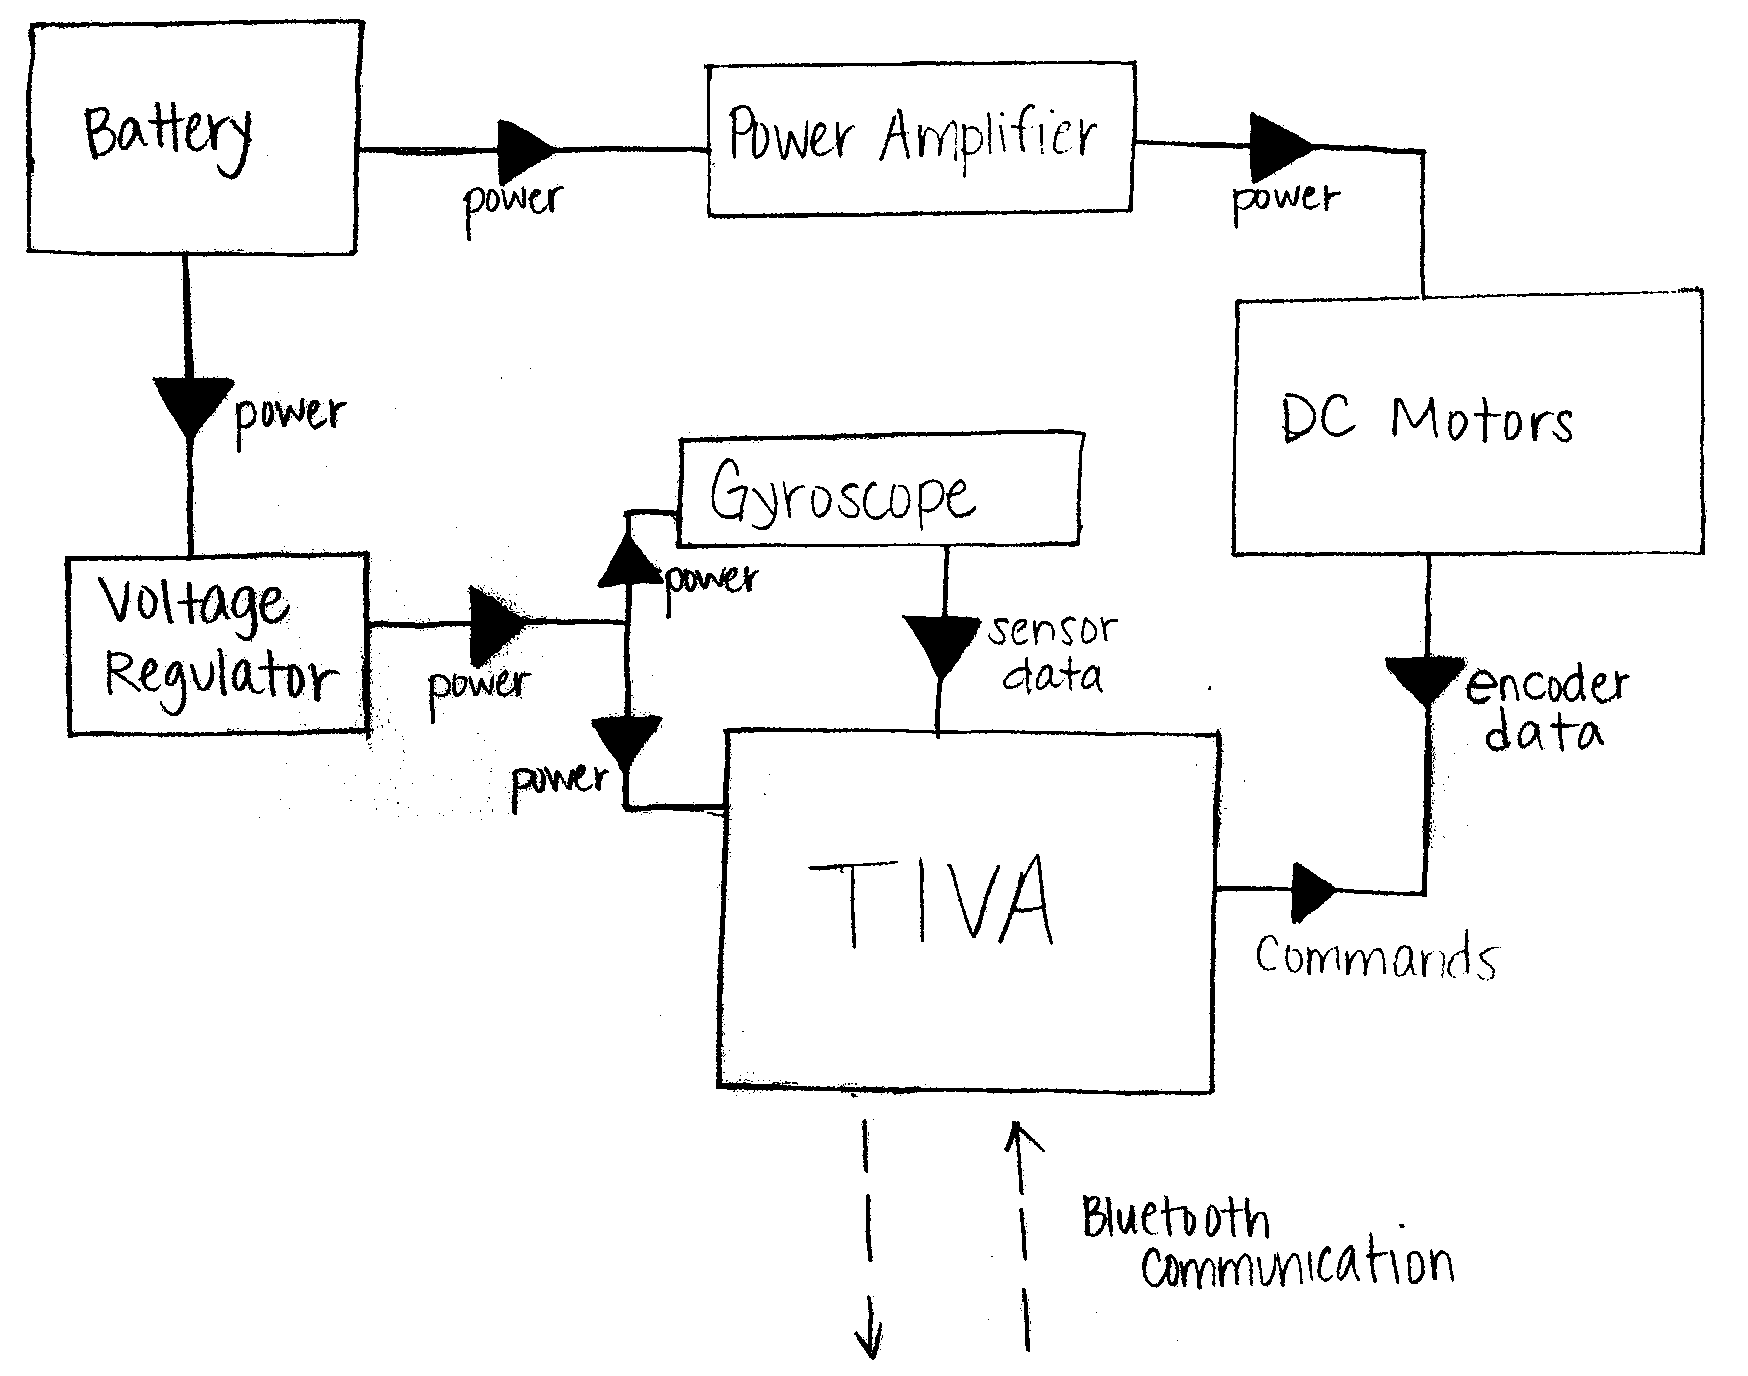
\includegraphics[width=0.5\textwidth]{BlockDiagram}
    \caption{Block Diagram of Subsystems}
    \label{BlockDiagram}
\end{figure}

\subsection*{Battery Subsystem}

For our standing robot, we would like to use battery packs to power the onboard computation, sensors, and the two torque motors that will enable the robot to self-balance. The final choice of exact battery pack will rely heavily on the motor test results that are gathered once we acquire and test the motor control in lab. As a preliminary estimation, it is expected that we will need a 9.6V or 12V NiMH (nickel metal-hydride) with a current rating somewhere between 2000 mAh and 10000 mAh. This prediction is based on the fact that similar size batteries are widely recommended for "small" robotics projects.

\subsection*{Wireless (Bluetooth\textsuperscript{\textregistered}) Communications Subsystem}

As a design requirement, our robot must be controlled through a wireless interface.  We have selected Bluetooth\textsuperscript{\textregistered} as our wireless protocol so we would easily be able to connect different devices as controllers.  We will have a backup IR sensor installed on the device that may possibly be used for pairing devices.  We will be using a peripheral communication chip to control the wirless communication so as to free up processor time on the Tiva board to allow for more thorough sensor readings and calculations.

\subsection*{Microcontroller Subsystem}

The microcontroller subsystem will consist of the Tiva board and will be responsible for bridging the various systems together. It will take input readings from the balancing and sensing subsystem and, based on the controller software implemented, produce an output to be used in the motor subsystem. Additionally, the microcontroller subsystem will interact with the wireless communications subsystem to receive user input about desired direction, turning, and powering down.

\subsection*{Balancing and Sensing Subsystem}

The purpose of the balancing system is to ensure that the robotic system will maintain a desired position determined by the microcontroller subsystem.  The desired position, called the desired $\theta_2$ value as shown in \cite{Groff}, is used as an input to the balancing system by the microcontroller subsystem.   The actual angle position of the robotic system is derived by measurements from a gyroscope.  The gyroscope measures angular velocity.  This value is then integrated twice to provide the actual angle position $\theta_2$.   The balancing system will then employ a PID control scheme to minimize the distance between the desired $\theta_2$ and the actual $\theta_2$ (i.e. minimizing the error).  To balance the system at rest, the desired $\theta_2$ will be set to zero.  To move the robot either forwards or backwards, the desired $\theta_2$ will be set to a positive or negative angle respectively.  This angle will be determined upon experimentation of the physical system.   The PID controller will send a signal back to the microcontroller subsystem to create a current signal to be fed to the motors.  Additionally, the built in encoders from the motors will be used to determine how much current is being applied to the motors.  The number of encoder counts in a certain amount of time will be used to determine the output torque of the motor and thus the applied current to achieve this torque.

\subsection*{Motor Subsystem}

The motor subsystem will consist of two continuous DC motors attached to each wheel of the Segway robot. The two motors will work together to balance the robot and move it as commanded by the controller. Moving straight or backwards will require both motors to exert the same torque in the same direction simultaneously, while turning will necessitate the motors moving at two different speeds (exerting two separate torques).  In order to balance while moving forward, the robot will first move backwards slightly to tilt the robot forward and "chase" itself to balance properly.

The motor subsystem will connect directly to the microcontroller subsystem and the power amplifier. The amplifier will augment the power supplied by the battery in order to sufficiently supply the motors. The microcontroller subsystem will receive data from the motors’ encoders and feed it back to the controls to be used in verifying the system’s current position. In return, the microcontroller subsystem will adjust the signals sent to each motor to govern their movement according to the desired motion provided by the controls. The DC 29:1 gear motors will exert a maximum torque of 8 kg cm$^2$ that will enable the Segway robot to reach a desired speed between 0.5 m/s and 1 m/s.  Together both motors will weigh no more than 0.84 pounds and will act as balancing weights on the bottom axle of the mechanical system.

\subsection*{Power Subsystem}

The batteries will be connected to the power amplifier. This amplifier will consist of two B547 transistors, one LED, and several resistors. This will allow the power to be amplified before going to the motors to ensure that proper torque is attained to drive the system. However, this system will not be connected to the Tiva board. The battery pack will also be wired to the voltage regulator chip. This will step down the voltage from the battery to 3.3 V. Regulating the voltage down to the proper level will ensure that the Tiva board does not receive too much voltage and stop working.

\subsection*{Mechanical Subsystem}

\begin{figure}[H]
    \centering
    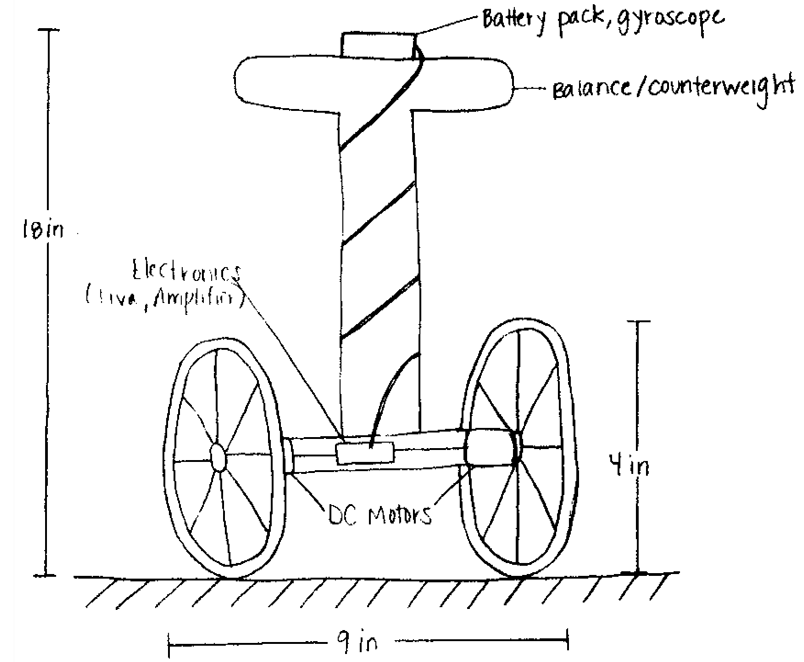
\includegraphics[width=0.5\textwidth]{PhysicalSystem}
    \caption{Physical System Drawing}
    \label{PhysicalSystem}
\end{figure}

The physical system is depicted in Figure \ref{PhysicalSystem}.  The robot will stand approximately eighteen inches tall with wheels approximately four inches in diameter.  The two wheels will lie on a shared axis approximately nine inches apart.  The two wheels will each be controlled independently of one another by separate DC motors.  The center part of the robot will be made from a light material like a PVC pipe.  The top of the robot will be a platform that acts as a counterweight and will hold the battery pack and gyroscope.  Also on this platform, bumpers will be included to protect the components mounted on the top in case of impact.  All of the other subsystems will be contained within the framework of the physical system.  There will also be a kickstand on the rear of the robot that will allow the robot to come to rest without having to constantly balance.  


\section*{Research and Analysis} %(1-3 pages)

\subsection*{Battery Power Supply}

There are multiple battery sizes and types available on the market. Many factors need to be taken into consideration to determine the correct battery for the correct application. In our case, a small multiple motor robot, a safe, cheap battery with a high energy density is needed. Lithium Ion Polymer batteries have a high energy density and small size, but they can be potentially dangerous. Lithium Ion batteries (common in laptops) can store lots of energy, but have relatively low current outputs, and are often quite expensive. Nickel Metal Hydride (NiMH) batteries are cheap, high energy density batteries that contain no toxic metals. This makes them a safer alternative to other options. There are many NiMH cells available for consumer use on the market, and lots of DIY projects recommend the use of NiMH battery packs. Given this information, our design will likely incorporate an NiMH battery pack as the onboard power supply \cite{Calin}.

\subsection*{Bluetooth\textsuperscript{\textregistered} Communication}

Bluetooth\textsuperscript{\textregistered} is a highly popular wireless communication standard.  By implementing Bluetooth\textsuperscript{\textregistered} in our system we greatly increase the portability and reliability of our robot.  There are many advantages to using Bluetooth\textsuperscript{\textregistered} over other protocols, such as IR technology.  The two major advantages of Bluetooth\textsuperscript{\textregistered} are that it does not require line of sight for communication and it can be readily modified to our needs using existing libraries and technologies.

We have decided to use the Emmoco EDB-BLE development board to control our wireless communications.  This board will allow us to utilize the Bluetooth\textsuperscript{\textregistered} 4.0 or Bluetooth\textsuperscript{\textregistered} Low Energy (BLE) standard, which will be useful for extending the battery life of our robot \cite{Nokia}.  By having a separate development board for Bluetooth\textsuperscript{\textregistered} communications we will be able to debug the wireless protocols seperately from the rest of the system.  This will save us development time and costs.

Additionally, Bluetooth\textsuperscript{\textregistered} technology offers multiple communication channels.  By using the Bluetooth\textsuperscript{\textregistered} stack we can stay connected to multiple control devices simultaneously.  This means that we can have multiple remote controllers for the system.  The EDB-BLE development board provides the em-framework which will allow our team to build custom control apps for moobile devices such as Android and iOS phones.

\subsection*{Wireless controller (Sony Dualshock 3\textsuperscript{\textregistered}) and Interfacing}

One of our goals is to fully interface with the Sony Dualshock 3\textsuperscript{\textregistered} controller system.  This will provide us with 2 10-bit joystick inputs, a 3-axis gyroscope, and 3-axis accelerometer for use as a controller.  We will be able to provide very detailed instructions to our robot so that the human-to-machine interfacing will feel natural and smooth.  If possible, we will try to integrate the rotational orientation and translational acceleration readings from the controller to produce a hybrid-control model.  This will allow to the user to not only direct the robot, but to "guide" the robot from a distance through natural motion.

\subsection*{Power Amplifier}

Researching the power amplifier yielded mixed results about how to build an amplifier that is both simple and functional. Two potential choices were determined: an amplifier built using operational amplifiers and an amplifier built using transistors and resistors. We decided to build an amplifier using transistors due to low cost and heating concerns.  The research indicated that in some cases the operational amplifiers became overheated very quickly. Because this project demands continued movement, excessive heat may not only affect the amplifier but also the temperature of the surrounding electronics. The two B547 transistors in combination with several bias resistors and an LED should create a functioning amplifier that is simple and inexpensive to replace should parts overheat and cease functional operation.

\subsection*{Voltage Regulators}

Due to the restrictions outlined in the project requirements, only one continuous DC voltage is permitted to power all electronics. This creates an issue because, while the Tiva is rated to operate at 3.3 V, the DC motors must run at a higher voltage in order to obtain the necessary torque. Therefore, a voltage regulator will be placed between the battery and Tiva chip. The Pololu Step Down Voltage Regulator D15V35F5S3 takes an input voltage between 4.5 and 24 V DC and can output either 3.3 or 5 V. This allows us to select the 3.3 V output and power the Tiva without worrying about damaging the controller. It also allows the motors to be run at a higher voltage than the controller to gain more torque for more robust movement. 

\subsection*{Motors}

There are three types of DC motors that are commonly used in robotics: continuous DC motors, stepper motors, and RC servo motors. Servo motors are not suitable for the two wheeled design without modification (and are not allowed anyway according to the project requirements). Stepper motors are incredibly accurate but not desirable for continuous motion or motion over uneven surfaces. Although our design will be moving over “flat” surfaces, there will still be small irregularities that it will need to overcome. We decided to use continuous DC motors with a low gear ratio (29:1) to ensure maximum achievable torque. By using motors with encoders, the position of the motors can be sent to the microcontroller subsystem and used to verify the balancing controls being sent to the motors. DC motors should provide the necessary torque as well as the range of motion that is desired.

\subsection*{PID Control}

The control scheme to be used in this system is a PID controller as shown in Figure \ref{PIDControlScheme} and defined analytically in Equation \ref{PIDControlEquation}.  This controller was chosen because it is relatively simple to tune and provides fine control.  A PID controller calculates an error signal by subtracting the actual measured value from the desired set value.  For this project, the desired set value is an angle called $\theta_2$, the angle between the zero position and the robot’s position.  The actual value is determined by integrating the output of a gyroscope sensor twice, from angular velocity to angular displacement.  This actual value is fed back to controller to determine the error signal.

\begin{figure}[H]
    \centering
    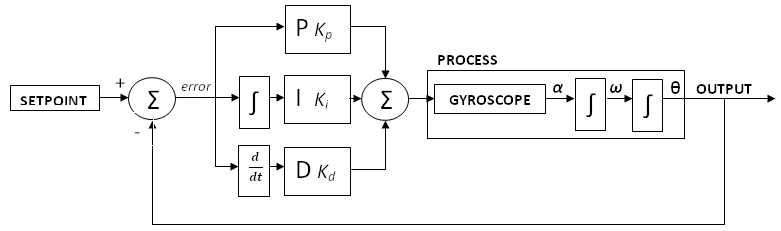
\includegraphics[width=0.7\textwidth]{PIDControlScheme}
    \caption{PID Control Scheme}
    \label{PIDControlScheme}
\end{figure}

\begin{align}
    u(t) &= \text{MV}(t) = K_p e(t) + K_i \int\limits_0^t e(\tau) d\tau + K_d \dfrac{d}{dt} e(t) \label{PIDControlEquation}
\end{align}

The PID controller is comprised of three gains: $K_p$, the proportional gain, $K_i$, the integral gain, and $K_d$, the derivative gain.  These three gains are used to reduce certain aspects of the error signal.  The proportional term yields an output that is directly proportional to the current error and as such is used to reduce present error.  Adjusting the proportional gain yields the most change to the output signal.  The integral term sums the instantaneous error over time and thus gives the accumulated offset that was not corrected for.  The integral term is used to eliminate the steady-state error left over from adjusting the proportional gain. The derivative term is used to predict the systems’ behavior and determine the future error.  The derivative gain is most useful in systems with little noise because excessive measurement noise will degrade the controller performance.   If any of these gains are set too high, the system is driven to instability.  To manually tune these gains, first the proportional gain is increased until the output signal begins to oscillate.  Then, the integral gain is increased until the output signal’s offset is corrected quickly.  Finally, if necessary, the derivative gain is increased so that the output signal will quickly reach zero.  Once our system’s controller gains are tuned, the output signal will then be sent to the motors as a current signal to control the motors.          
                                                                                                                                                                                                                                                                                                                                                                                                                                                                                               
To ensure that the task of tuning the gains for the controller is kept as simple as possible, the choice of motors to control the wheels of the robot is limited.  Specifically, the ideal choice of motor would be one without a gear box.  The more gears present in the gear box, the more difficult it becomes to tune the gains of the controller.

\subsection*{Gyroscopes}

The gyroscope we selected is a 9DOF MPU-9150 9-axis MotionTracking MEMS device.  It has a 3-axis accelerometer, 3-axis gyroscope, and 3-axis compass.  The 9DOF was specifically designed for low power, low cost, and high performance devices.  Full 9-axis operation will draw 4.25 mA with maximum gyro sampling, a 1kHz accelerometer sample rate, and an 8Hz compass sample rate.  The 9DOF is capable of reading $\pm2000$ degrees per second up to 131 LSBs/dps for the gyroscope.

By using such a highly tuned gyroscope, we will be able to quickly notice shifts in momentum and torque through the system.  This will allow for greater control over the device. Since this device can be tuned down for low power consumption, we can also extend battery life by turning off the compass and lowering the sampling rates for the remaining 6 axes.

\subsection*{Mechanical}

Shown in Figure \ref{MathDiagram} is the mathematical model that describes the system.  Four variables correspond to the wheel: $m_1$ is the mass, $I_1$ the moment of inertia, $r$ is the radius, and $\theta_1$ is the wheel angle.  $M_2$ is the mass and $I_2$ is the moment of inertia of the counter mass.  $L$ is the length from the axis to the center of mass of the counter mass and $\theta_2$ is the angle between the y axis and the body of the robot.  The transfer function for this system is given by $G_{\theta_2 T}$ shown in Figure \ref{TransferFunction}.

\begin{figure}[H]
    \centering
    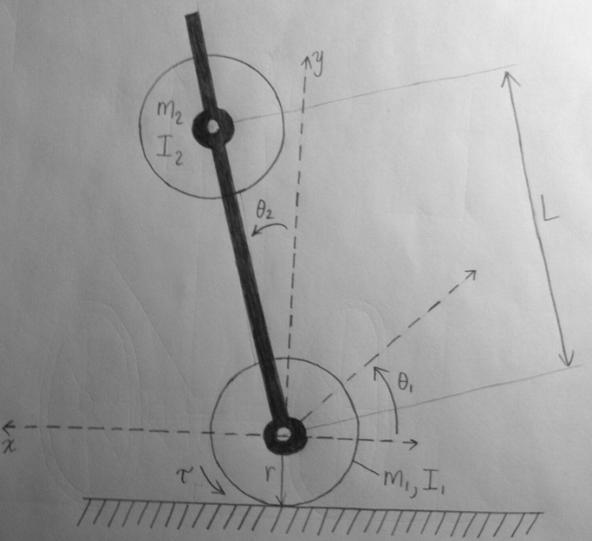
\includegraphics[width=0.5\textwidth]{MathDiagram}
    \caption{Mathematical Model}
    \label{MathDiagram}
\end{figure}

\begin{figure}[H]
    \centering
    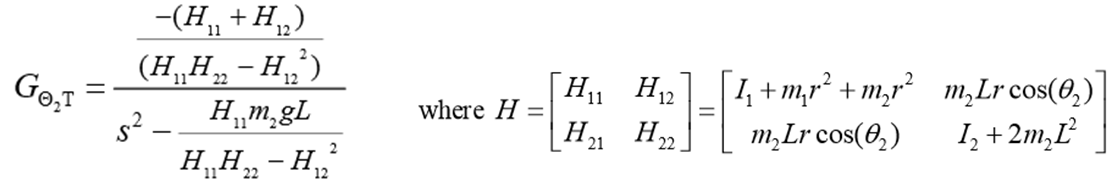
\includegraphics[width=0.75\textwidth]{TransferFunction}
    \caption{Transfer Function}
    \label{TransferFunction}
\end{figure}

As shown in the mathematical model, the transfer function will yield two poles, one of which is in the right half of the plane which leads to an unstable system.  In order to create a stable system, the poles must be moved to the left half of the plane.  The mechanical systems’ parameters can be changed in order to accomplish this goal.  Specifically, the two most practical adjustments that can be made to the model are to increase $L$ while also increasing $m_2$.  The idea is to get the mass of the robot as far from the ground in order to slow the movement of the robot, thus making the system easier to control.

\section*{Risk Assessment and Contingency Plans} %(1 page)

Safety should be one of the most important focuses of any project. For our project, we have identified potential hazards that could develop during the course of work. For any mechanical/fabrication work, there is always the possibility of shards/fragments/dust being expelled from the subject of work. In order to mitigate the potential eye damage, safety glasses are to be worn at all times when power tools are being used or there is ongoing testing involving moving parts. 

Batteries introduce another hazard in the form of fire and explosion. It is quite common for batteries to overheat, and this can lead to dangerous explosions or burn related injuries. External forces can also damage batteries – this can lead to leakage of toxic chemicals. To mitigate these dangers, the team is planning to use a NiMH battery to negate the presence of dangerous chemicals. During motor load testing, the maximum current draw will be determined. From there, we will determine if we need a fan or some other heat sink to cool the battery during operation. 

In the unlikely event that our battery fails or does not perform as expected, we plan on ordering a DC wall adapter to power the robot. While undesirable, a DC wall adapter provides a cheap way to ensure a power source in the case of an equipment malfunction. 

The team has also identified several bottlenecks in our project development. These subsystems will all be worked on in parallel to minimize the down-time experienced. The systems identified include: the power supply/electronics, the mechanical design, and the sensing system. Without the mechanical frame and gyroscopes being developed, it will be impossible to calibrate any kind of motor control, and none of these systems will work without a power supply. The plan is to start by using the bench top amplifier and DC supplies to power the initial stages of the project, and switch to using our own electronics after the first milestone. This will allow time for the proper theoretical design and parts acquisition to take place.  


\section*{Testing and Data Collection Plan} %(1.5 page)

\subsection*{Testing Plan}

\paragraph*{Balancing System}
The first tests that will be run for this subsystem will be testing the accuracy and robustness of the different sensors.  To test the gyroscope, the robot will be moved to different angles while the output of the gyroscope is recorded.  These measured angular velocities will be used to determine the desired values for the controller.  The encoders will be similarly tested.  The goal in this case is to determine the relationship between encoder counts and applied current (i.e. number of encoder counts will be used to determine how much current is being applied to the motor).    However, the majority of testing that will take place for this subsystem will come from the process of tuning the gains to write the PID controller.  A series of runs will be executed for each command (i.e. balance in position, move forward, turn, etc.).  While the system is running, different scopes will be used to compare the actual position with the desired position.  This data will be continually collected as the gains are adjusted to reduce the error.  

\paragraph*{Motors}
In order to test the functionality of the motors, two tests will be performed. For the preliminary torque test, the motors will be connected to the wheels and sent signals to move at different speeds. The speed of the rotating wheel will be visually observed and the control speeds will be calibrated in order to determine what needs to be sent to the motors to achieve minimum and maximum speeds. Additionally, timing tests will be performed to ascertain how quickly the motors react to directed signals. A huge component to being able to balance the robot well is how responsive the motors are once the control signals are sent. The motors must move and exert torque very quickly to correctly balance the system. Varying signals will be sent to the two motors and their response times will be recorded to gauge how well the motors will be able to respond and balance the system. 

\paragraph*{Power Amplifier and Voltage Regulator}
Both the power amplifier electronics and voltage regulator only need to be tested using a multimeter. The input voltages will be tested to verify their compatibility with the circuit components. Each electronic device will then be wired into the system and its voltage and current outputs measured before connecting them to the entire system. The resistors will need to be adjusted for the power amplifier based on these findings and the output of the voltage regulator must be verified at 3.3 V to ensure that it is a safe voltage to avoid damaging the Tiva microcontroller.

\paragraph*{Mechanical System}
The majority of the testing for this system will be to test for robustness and durability.  This testing is necessary to ensure that the more delicate parts of the overall system will be protected.  Experimentation will also be done with the length of the PVC pipe and the mass of the counterweight to determine the best configuration to ensure a safe, durable, and controllable system.

\subsection*{Data Collection Plan}

In order to preserve all the data concerning the proper function of the system, both videos and photos will be taken prior to each milestone to show that all required systems are properly operational. Additionally, plots for error control will be saved for future work and times for the balancing and speed components will be tested and recorded prior to each milestone. The system speed and time it takes to balance are important components to prove the practicality of the robot. Any overshoot will be measured if the signal is dropped.

\section*{Cost Accounting} %(1 page)

    {
    \centering
    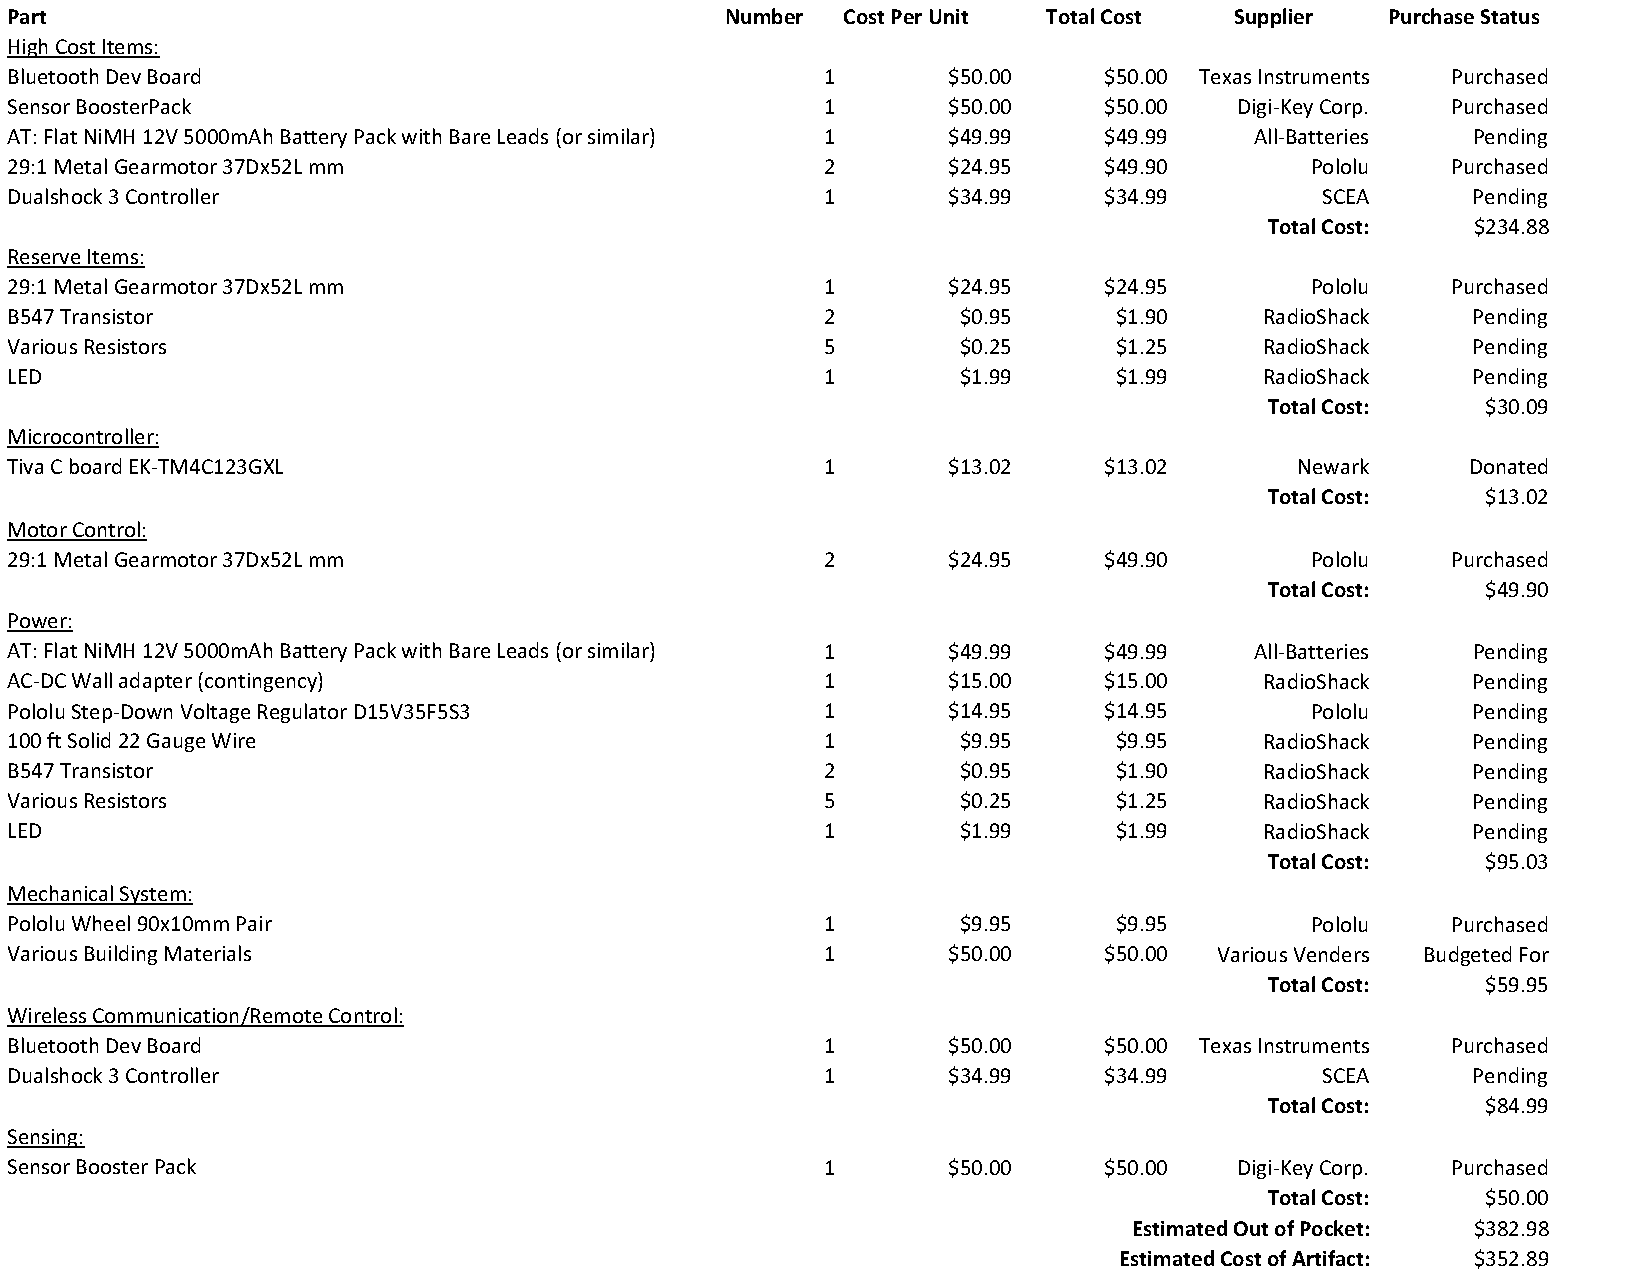
\includegraphics[width=\textwidth]{CostAccounting}
    }

\section*{Project Schedule} %(1 page)

\begin{tabular}{lllll}

Task & Start Date & End Date & Assigned To \\
\hline
Motor Control & Feb 3 & Feb 17 & Laura \\
Sensor System &	Feb 3 &	Feb 17 &			Katelyn \\
Structure	& Feb 3	& Feb 14 &			Katelyn, Greg \\
\textit{Milestone 1}	& Feb 17 &	Feb 17		\\		
Microcontroller System	& Feb 3	& Feb 21 &	 Julian, Ben \\
Bluetooth	& Feb 24 & 	Mar 13	& 	Julian, Ben \\
Stabilize System	& Feb 18	& Mar 3	 	& Katelyn \\
\textit{Milestone 2} &	Mar 3 &	Mar 3	 \\			
Battery Power	& Feb 17 &	Mar 20 &	 Laura, Greg \\
Tuning \& Calibration	& Mar 3	& Mar 24 &		Julian, Ben, Katelyn \\
\textit{Milestone 3}	& Mar 25	& Mar 25				 \\
Tweak	& Mar 25 &	Apr 7 &	Julian, Laura, Ben, Katelyn, Greg \\
\textit{Demo} & Apr 7 & Apr 7 \\				


\end{tabular}

% Bibliography
\bibliography{citationsfile}{}

\clearpage

\section*{Appendix A: Parts List}

\begin{tabular}{lll}
Supplier & Part Number & Quantity \\
\hline
RadioShack & 278-1215 & 1 \\
Pololu & 	1103	 & 3 \\
RadioShack & 57-12D-500-4 & 	1 \\
All-Battery & 	11626	 & 1 \\
RadioShack & 276-1617 & 2 \\
Texas Instruments & 	CC2560-PAN1325 & 	1 \\
SCEA & 	98464	 & 1 \\
RadioShack & NTE3140 & 1 \\
Pololu & 	 D15V35F5S3	 & 1 \\
Pololu & 	1435	 & 1 \\
Digi-Key Corp. & 	430BOOST-ADS1118 & 	1 \\
Newark & 	 EK-TM4C123GXL	 & 1 \\
Various Venders & 	N/A & 	1 \\
RadioShack & 271-309 & 5 \\
\end{tabular}


%% END EDITS HERE %%

\end{spacing}

\end{document}
